\PassOptionsToPackage{unicode}{hyperref}
\PassOptionsToPackage{hyphens}{url}
\PassOptionsToPackage{dvipsnames,svgnames,x11names}{xcolor}
%
\documentclass[11pt,english]{article}

\usepackage{amsmath,amssymb}
\usepackage{iftex}
\ifPDFTeX
  \usepackage[T1]{fontenc}
  \usepackage[utf8]{inputenc}
  \usepackage{textcomp}
\else
  \usepackage{unicode-math}
  \defaultfontfeatures{Scale=MatchLowercase}
  \defaultfontfeatures[\rmfamily]{Ligatures=TeX,Scale=1}
\fi
\usepackage{lmodern}
\usepackage{tabularx}
\IfFileExists{upquote.sty}{\usepackage{upquote}}{}
\IfFileExists{microtype.sty}{%
  \usepackage[]{microtype}
  \UseMicrotypeSet[protrusion]{basicmath}%
}{}
\makeatletter
\@ifundefined{KOMAClassName}{%
  \IfFileExists{parskip.sty}{%
    \usepackage{parskip}%
  }{%
    \setlength{\parindent}{0pt}
    \setlength{\parskip}{6pt plus 2pt minus 1pt}%
  }%
}{%
  \KOMAoptions{parskip=half}%
}
\makeatother
\usepackage[dvipsnames,svgnames,x11names]{xcolor}
\usepackage[margin=2.2cm]{geometry}
\usepackage{fancyvrb}
\newcommand{\VerbBar}{|}
\newcommand{\VERB}{\Verb[commandchars=\\\{\}]}
\DefineVerbatimEnvironment{Highlighting}{Verbatim}{commandchars=\\\{\}}
\newenvironment{Shaded}{}{}
\usepackage{longtable,booktabs,array}
\usepackage{calc}
\usepackage{etoolbox}
\makeatletter
\patchcmd\longtable{\par}{\if@noskipsec\mbox{}\fi\par}{}{}
\makeatother
\IfFileExists{footnotehyper.sty}{%
  \usepackage{footnotehyper}%
}{%
  \usepackage{footnote}%
}
\makesavenoteenv{longtable}
\usepackage{graphicx}
\makeatletter
\def\maxwidth{%
  \ifdim\Gin@nat@width>\linewidth
    \linewidth
  \else
    \Gin@nat@width
  \fi
}
\def\maxheight{%
  \ifdim\Gin@nat@height>\textheight
    \textheight
  \else
    \Gin@nat@height
  \fi
}
\makeatother
\setkeys{Gin}{width=\maxwidth,height=\maxheight,keepaspectratio}
\makeatletter
\def\fps@figure{htbp}
\makeatother
\setlength{\emergencystretch}{3em}
\providecommand{\tightlist}{%
  \setlength{\itemsep}{0pt}\setlength{\parskip}{0pt}}
\setcounter{secnumdepth}{-\maxdimen}
\ifLuaTeX
  \usepackage{selnolig}
\fi
\IfFileExists{bookmark.sty}{%
  \usepackage{bookmark}%
}{%
  \usepackage{hyperref}%
}
\IfFileExists{xurl.sty}{\usepackage{xurl}}{}
\urlstyle{same}
\hypersetup{
  pdftitle={Terrain-Induced Slugging in OpenFOAM: static verification (dip2D\_hydrostatic\_n10)},
  colorlinks=true,
  linkcolor={blue},
  filecolor={Maroon},
  citecolor={Blue},
  urlcolor={blue},
  pdfcreator={LaTeX}}

\usepackage{fancyhdr}
\pagestyle{fancy}
\setlength{\headheight}{14pt}
\lhead{Skoltech. F2026. Modeling with Open Source Software. Project report.}
\rhead{By Arofenitra Rarivonjy}
\renewcommand{\headrulewidth}{1pt}

\date{}
\AtBeginDocument{%
  \def\labelitemi{\(\diamond\)}%
}

\usepackage{babel}

\begin{document}

\title{Terrain-Induced Slugging in OpenFOAM\\
{\large{}A term project in the course: Modeling with Open Source Software}}
\author{by Arofenitra Rarivonjy, Skoltech, Fall 2026}
\maketitle

\begin{abstract}
The case presented in this project progress report is about \textbf{static verification} of a two-phase solver on a V-shaped geometry pipe, where the liquid pool is initialised in exact hydrostatic equilibrium with closed inlets so that any residual motion is a numerical artefact. The hydrostatic pressure is reproduced to 0.01\,\%. The composite source $S_\alpha$ has a zero explicit mass-transfer part, while cycle-resolved grid and time-step convergence remain to be demonstrated.
\end{abstract}
{
\hypersetup{linkcolor=}
\setcounter{tocdepth}{2}
\tableofcontents
}

\section{1. Problem description and motivation}\label{problem-description-and-motivation}

This case is a \textbf{static verification} of the two-phase solver on
the dip geometry. The liquid pool is initialised in exact hydrostatic
equilibrium and both inlets are closed (zero prescribed velocity), so
the exact solution is: velocity identically zero, pressure hydrostatic
in each phase, and a flat liquid/gas interface. Any non-zero velocity or
pressure drift is a numerical artefact and is measured here.

Motivation: before trusting a dynamic slugging simulation, the same mesh
and scheme must reproduce a state that should not move. This separates
discretisation errors (spurious currents at the density jump,
pressure-velocity decoupling) from physical dynamics.

\section{2. Mathematical formulation}\label{mathematical-formulation}

\subsection{2.1 Governing equations}\label{governing-equations}

The solver is OpenFOAM-14 \texttt{compressibleVoF}, run by
\texttt{foamRun}. Unknowns are one velocity \(\mathbf U\), pressure
\(p\), temperature \(T\) and the liquid fraction \(\alpha_l\)
(\texttt{0/alpha.oil}, \(\alpha_g=1-\alpha_l\)), with
\(\rho=\alpha_l\rho_l+\alpha_g\rho_g\),
\(\mu=\alpha_l\mu_l+\alpha_g\mu_g\), \(\rho_g=p/(R_gT)\) (perfect gas)
and \(\rho_l\) constant (\texttt{rhoConst}). The governing equations stem
from the mass/volume balance of the two-phase mixture, liquid-phase
transport, momentum (local mixture density, pressure, gravity, viscous
stress, surface tension) and energy (storage and advection of internal
and kinetic energy, diffusion):

\[
\begin{aligned}
\partial_t \rho + \nabla\cdot(\rho\mathbf U) &= 0,\\
\partial_t(\alpha_l\rho_l)+\nabla\cdot(\alpha_l\rho_l\mathbf U)
+\nabla\cdot(\alpha_l\alpha_g\rho_l\mathbf U_r) &= S_\alpha,\\
\partial_t(\rho\mathbf U)+\nabla\cdot(\rho\mathbf U\mathbf U)
&= -\nabla p+\rho\mathbf g+\nabla\cdot\boldsymbol\tau+\sigma\kappa\nabla\alpha_l,\\
\partial_t(\rho e)+\nabla\cdot(\rho\mathbf U e)+\partial_t(\rho K)+\nabla\cdot(\rho\mathbf U K)
&= \nabla\cdot(\alpha_{eff}\nabla T),
\end{aligned}
\]

with the interface-compression velocity
\(\mathbf U_r=c_\alpha|\mathbf U|\hat{\mathbf n}\), \(c_\alpha=1\),
\(\hat{\mathbf n}=\nabla\alpha_l/|\nabla\alpha_l|\), the curvature
\(\kappa=-\nabla\cdot\hat{\mathbf n}\) of the CSF model and the
compressibility source \(S_\alpha\). The energy equation is what makes
the gas response close to adiabatic.

\subsection{2.2 Modelling assumptions}\label{modelling-assumptions}

\begin{itemize}
\tightlist
\item
  Inlets closed (velocity fixed to zero), outlet pressure fixed: no
  forced throughflow.
\item
  Initial pressure is hydrostatic in the liquid:
  \texttt{p\_rgh\ =\ p0\ +\ (rho\_l\ -\ rho\_g)\ g\ y\_s}; a uniform
  p\_rgh would introduce a spurious 1.3 kPa step at the interface.
\item
  Surface tension is active in the baseline; the sigma = 0 twin
  (separate case) isolates the capillary contribution to the parasitic
  current.
\item
  Laminar; no turbulence model. Density ratio 750:1 and viscosity ratio
  1.1e4:1 as in production.
\end{itemize}

\subsection{2.3 Initial and boundary conditions}\label{initial-and-boundary-conditions}

Boundary-condition \textbf{types} can be verified in the \texttt{0/}
dictionaries:

\begin{table}[htbp]
\centering
\small
\renewcommand{\arraystretch}{1.3}
\begin{tabularx}{\textwidth}{@{}l *{4}{>{\centering\arraybackslash}X} c@{}}
\toprule
patch & U & p\_rgh & alpha.oil & T & p \\
\midrule
inletLiquid  & fixedValue & fixedFluxPressure & fixedValue & fixedValue & calculated \\
inletGas     & fixedValue & fixedFluxPressure & fixedValue & fixedValue & calculated \\
outlet       & \shortstack{pressureInlet\\OutletVelocity} & fixedValue & inletOutlet & inletOutlet & calculated \\
walls        & noSlip & fixedFluxPressure & zeroGradient & zeroGradient & calculated \\
frontAndBack & empty  & empty & empty & empty & empty \\
\bottomrule
\end{tabularx}
\end{table}

\begin{longtable}[]{@{}
  >{\raggedright\arraybackslash}p{(\columnwidth - 2\tabcolsep) * \real{0.5000}}
  >{\raggedright\arraybackslash}p{(\columnwidth - 2\tabcolsep) * \real{0.5000}}@{}}
\toprule\noalign{}
\begin{minipage}[b]{\linewidth}\raggedright
type
\end{minipage} & \begin{minipage}[b]{\linewidth}\raggedright
meaning
\end{minipage} \\
\midrule\noalign{}
\endhead
\bottomrule\noalign{}
\endlastfoot
\texttt{fixedValue} & impose the value (velocity, phase fraction,
temperature, or the pressure level at the outlet) \\
\texttt{fixedFluxPressure} & adjust the pressure so the mass flux
matches the velocity BC (walls and velocity inlets) \\
\texttt{pressureInletOutletVelocity} & zero velocity unless the flow
wants to enter, then it follows the pressure \\
\texttt{inletOutlet} & zero gradient for outflow, fixed inlet value for
backflow \\
\texttt{calculated} & recomputed from other fields (p = p\_rgh +
rho*gh) \\
\texttt{zeroGradient} & no normal gradient (adiabatic wall for T) \\
\texttt{noSlip} & zero velocity at the wall \\
\texttt{empty} & 2D constraint: the solution does not vary through this
direction \\
\end{longtable}

Initial condition (\texttt{system/setFieldsDict}):

\begin{verbatim}
defaultValues
{
    alpha.oil     0;
    p_rgh       100000;
}

zones
{
    // horizontal free surface at y = 0.15 m: liquid below, gas above
    pool
    {
        type        box;
        box         (-1e300 -1e300 -1e300) (1e300 0.15 1e300);
        values
        {
            alpha.oil     1;
            p_rgh       101322.5842;
        }
    }
}
\end{verbatim}

The liquid is initialised with the exact hydrostatic \texttt{p\_rgh}
(\texttt{p\_rgh\ =\ p0\ +\ (rho\_l\ -\ rho\_g)\ g\ y\_s}) instead of a
uniform value, which makes the initial state static to round-off in the
liquid.

\section{3. Dimensional analysis}\label{dimensional-analysis}

\subsection{3.1 Length and grid scales}\label{length-and-grid-scales}

\begin{longtable}[]{@{}
  >{\raggedright\arraybackslash}p{(\columnwidth - 6\tabcolsep) * \real{0.2500}}
  >{\raggedright\arraybackslash}p{(\columnwidth - 6\tabcolsep) * \real{0.2500}}
  >{\raggedright\arraybackslash}p{(\columnwidth - 6\tabcolsep) * \real{0.2500}}
  >{\raggedright\arraybackslash}p{(\columnwidth - 6\tabcolsep) * \real{0.2500}}@{}}
\toprule\noalign{}
\begin{minipage}[b]{\linewidth}\raggedright
scale
\end{minipage} & \begin{minipage}[b]{\linewidth}\raggedright
definition
\end{minipage} & \begin{minipage}[b]{\linewidth}\raggedright
value
\end{minipage} & \begin{minipage}[b]{\linewidth}\raggedright
significance
\end{minipage} \\
\midrule\noalign{}
\endhead
\bottomrule\noalign{}
\endlastfoot
diameter / gap D & given & 0.05 m & pipe diameter, also the grid
scale \\
vertical height H & D/cos(theta) & 0.05019 m & 2D planar channel
height \\
total length L & 2 x 3 m & 6 m & L/D = 120 \\
dip depth dz & L\_leg sin(theta) & 0.2615 m & sets the hydrostatic head
rho\_l g dz = 2.308 kPa \\
grid spacing & D/n & 5.000 mm & D/dx = 10 \\
vertical spacing & H/n & 5.019 mm & 10 cells across H \\
capillary length & sqrt(sigma/(Delta rho g)) & 1.84 mm & below grid
scale: capillarity under-resolved \\
\end{longtable}

\subsection{3.2 Time scales}\label{time-scales}

\begin{longtable}[]{@{}
  >{\raggedright\arraybackslash}p{(\columnwidth - 6\tabcolsep) * \real{0.2500}}
  >{\raggedright\arraybackslash}p{(\columnwidth - 6\tabcolsep) * \real{0.2500}}
  >{\raggedright\arraybackslash}p{(\columnwidth - 6\tabcolsep) * \real{0.2500}}
  >{\raggedright\arraybackslash}p{(\columnwidth - 6\tabcolsep) * \real{0.2500}}@{}}
\toprule\noalign{}
\begin{minipage}[b]{\linewidth}\raggedright
scale
\end{minipage} & \begin{minipage}[b]{\linewidth}\raggedright
definition
\end{minipage} & \begin{minipage}[b]{\linewidth}\raggedright
value
\end{minipage} & \begin{minipage}[b]{\linewidth}\raggedright
significance
\end{minipage} \\
\midrule\noalign{}
\endhead
\bottomrule\noalign{}
\endlastfoot
advective & D/(J\_L+J\_G) & 0.07143 s & cell-crossing time \\
system transit & L/(J\_L+J\_G) & 8.571 s & through-flow time \\
leg transit & L\_leg/J\_G & 6 s & gas displacement time \\
acoustic transit & L/c & 0.01749 s & pressure equilibration (c = 343.1
m/s) \\
gas compression & L\_leg/J\_G & 6 s & time to compress the trapped
gas \\
viscous diffusion (oil) & D\^{}2/nu\_l & 11.25 s & momentum diffusion
across the channel \\
viscous film & h\^{}2/nu\_l & 1.012 s & h = 0.3 D inlet layer \\
tilted U-tube & 2 pi sqrt(L/(2 g sin theta)) & 11.77 s & gravity-wave
scale of the liquid column \\
simulated time & endTime & 5 s & see results for how many cycles \\
\end{longtable}

\subsection{3.3 Dimensionless groups}\label{dimensionless-groups}

\begin{longtable}[]{@{}
  >{\raggedright\arraybackslash}p{(\columnwidth - 6\tabcolsep) * \real{0.2500}}
  >{\raggedright\arraybackslash}p{(\columnwidth - 6\tabcolsep) * \real{0.2500}}
  >{\raggedright\arraybackslash}p{(\columnwidth - 6\tabcolsep) * \real{0.2500}}
  >{\raggedright\arraybackslash}p{(\columnwidth - 6\tabcolsep) * \real{0.2500}}@{}}
\toprule\noalign{}
\begin{minipage}[b]{\linewidth}\raggedright
group
\end{minipage} & \begin{minipage}[b]{\linewidth}\raggedright
definition
\end{minipage} & \begin{minipage}[b]{\linewidth}\raggedright
value
\end{minipage} & \begin{minipage}[b]{\linewidth}\raggedright
physical significance
\end{minipage} \\
\midrule\noalign{}
\endhead
\bottomrule\noalign{}
\endlastfoot
Re\_sl & rho\_l J\_L D/mu\_l & 45.0 & liquid superficial Reynolds:
laminar \\
Re\_sg & rho\_g J\_G D/mu\_g & 1666.7 & gas superficial Reynolds: at the
laminar/transitional edge \\
Re\_g,local & rho\_g U\_g D/mu\_g & 2381 & in-situ gas Reynolds just
above 2300 (assumption: laminar) \\
Fr\_m & (J\_L+J\_G)/sqrt(gD) & 0.9995 & inertia vs gravity; Fr
\textasciitilde{} 1 \\
Eo & Delta rho g D\^{}2/sigma & 734.8 & gravity dominates capillarity by
\textasciitilde700 \\
We\_g & rho\_g J\_G\^{}2 D/sigma & 0.5 & gas inertia vs capillarity
(weak) \\
rho\_l/rho\_g & - & 750 & density ratio: the hard VOF number \\
mu\_l/mu\_g & - & 11111 & viscosity ratio \\
rho\_l g dz/p0 & - & 0.02308 & compression parameter: 2.3 \%
(compressibility matters) \\
L/D & - & 120 & slug length 12-30 D fits 4-10 times \\
l\_c/D & - & 0.03689 & capillary length / gap \\
\end{longtable}

\subsection{3.4 Interpretation}\label{interpretation}

The liquid is laminar (\texttt{Re\_sl\ =\ 45}); the gas sits at the
laminar/transitional edge
(\texttt{Re\_g,local\ \textasciitilde{}\ 2.4e3}), which is an
assumption. \texttt{Eo\ \textasciitilde{}\ 735} means gravity dominates
surface tension by nearly three orders of magnitude, so the interface
shape is gravity-controlled.
\texttt{Fr\_m\ \textasciitilde{}\ 1} means inertia and
gravity are comparable, so neither can be neglected. The
\textbf{compression parameter \texttt{rho\_l\ g\ dz/p0\ =\ 2.3\ \%}} is
the key number for this problem: it is small enough that the flow looks
almost incompressible, but large enough that the dip stores a measurable
gas pressure, which is exactly why the compressible-VOF model is
needed. The density ratio 750 is what makes the VOF interface and the
pressure-gradient balance numerically hard.

\section{4. Numerical methodology and expected accuracy}\label{numerical-methodology-and-expected-accuracy}

\subsection{4.1 Discretisation}\label{discretisation}

The solver is OpenFOAM-14 \texttt{compressibleVoF}, run by
\texttt{foamRun}. It uses the \textbf{finite-volume method} on a
structured hexahedral mesh. For a conserved quantity \(\phi\) in control
volume \(V_P\) with faces \(f\),

\[
\int_{V_P}\partial_t\phi\,dV + \oint_{\partial V_P}\mathbf F\cdot d\mathbf A
= \int_{V_P}S\,dV
\quad\Longrightarrow\quad
\partial_t(\phi_P V_P) + \sum_f F_f A_f = S_P V_P ,
\]

with the face flux \(F_f = \mathbf U_f\cdot\mathbf n_f\) evaluated by
linear (central) interpolation and the face value \(\phi_f\) by the
selected convection scheme:

\begin{itemize}
\tightlist
\item
  \textbf{first-order upwind} (used for \(\mathbf U\) and \(T\)):
  \(\phi_f = \phi_{UP}\), stable but numerically diffusive
  (\(\mathcal O(h)\) on smooth fields);
\item
  \textbf{linear/central} for gradients and the pressure term, second
  order on smooth fields;
\item
  \textbf{interface compression} for the phase fraction: a flux
  \(\alpha_l\alpha_g\mathbf U_r\) with
  \(\mathbf U_r = c_\alpha|\mathbf U|\hat{\mathbf n}\), \(c_\alpha=1\),
  \(\hat{\mathbf n}=\nabla\alpha_l/|\nabla\alpha_l|\), which sharpens
  the interface while preserving boundedness.
\end{itemize}

\emph{Time}: first-order implicit Euler,
\(\phi^{n+1}=\phi^n+\Delta t\,f(\phi^{n+1})\), with the time step
controlled by \texttt{adjustTimeStep} and the Courant number

\[
\mathrm{Co} = \max_f \frac{|\phi_f|\Delta t}{V_P} \le 0.5,\qquad
\mathrm{Co}_\alpha = \max_f \frac{|\phi_{\alpha,f}|\Delta t}{V_P} \le 0.5 .
\]

The phase fraction is advanced with \textbf{MULES}: an explicit
flux-limited update

\[
\alpha_P^{n+1} = \alpha_P^{n} - \frac{\Delta t}{V_P}\sum_f \lambda_f F_{\alpha,f},
\qquad \lambda_f \in [0,1],
\]

where the limiter \(\lambda_f\) is chosen so that \(0\le\alpha\le1\);
\texttt{nSubCycles} sub-cycles keep \(\mathrm{Co}_\alpha\le 0.5\). The
pressure-velocity coupling is \textbf{PIMPLE} (a merged PISO/SIMPLE):
after the momentum equation the pressure correction \(p'\) solves
\(\nabla\cdot\left(A_p^{-1}\nabla p'\right) = \nabla\cdot\mathbf U^* + \text{compressibility source}\),
the velocity is corrected as
\(\mathbf U=\mathbf U^* - A_p^{-1}\nabla p'\), and the loop is repeated
\texttt{nOuterCorrectors} times. For compressible flow the continuity
equation carries the density compressibility
\(\psi=\partial\rho/\partial p = 1/(R_gT)\), which is how the dip stores
gas pressure.

\emph{Expected accuracy}: second order in space for smooth fields
(central terms), first order in time (Euler), and \textbf{first order
for the interface position} because the VOF interface is 1-2 cells
thick; the effective order of the global pressure history is therefore
\(\approx 1\)--\(2\).

\subsection{4.2 Solver controls}\label{solver-controls}

\begin{longtable}[]{@{}
  >{\raggedright\arraybackslash}p{(\columnwidth - 2\tabcolsep) * \real{0.5000}}
  >{\raggedright\arraybackslash}p{(\columnwidth - 2\tabcolsep) * \real{0.5000}}@{}}
\toprule\noalign{}
\begin{minipage}[b]{\linewidth}\raggedright
setting
\end{minipage} & \begin{minipage}[b]{\linewidth}\raggedright
value
\end{minipage} \\
\midrule\noalign{}
\endhead
\bottomrule\noalign{}
\endlastfoot
solver & compressibleVoF \\
time scheme & Euler \\
U convection & Gauss upwind \\
nOuterCorrectors / nCorrectors & 2 / 1 \\
MULES nSubCycles / nIter & 2 / 5 \\
maxCo / maxAlphaCo & 0.5 / 0.5 \\
maxDeltaT {[}s{]} & 0.01 \\
endTime {[}s{]} / writeInterval {[}s{]} & 5 / 0.25 \\
function objects & probes, interfaceHeight1, totalMass, maxU, massIn,
massOut, pOutlet \\
\end{longtable}

\subsection{4.3 Expected accuracy and error sources}\label{expected-accuracy-and-error-sources}

\begin{itemize}
\tightlist
\item
  Spatial: formally second order for the central terms, \textbf{first
  order for U and T} (upwind), and first order for the interface
  position because the VOF interface is 1-2 cells thick.
\item
  Temporal: first-order Euler; the time step is capped by
  \texttt{Co\ \textless{}=\ 0.5} and
  \texttt{Co\_alpha\ \textless{}=\ 0.5}, so the temporal error is
  expected to be small.
\item
  Linear-solver error: pressure tolerance 1e-8 (relative),
  velocity/alpha tight tolerances; the solver converges every time step
  (\texttt{nOuterCorrectors} PIMPLE loops).
\item
  Modelling errors dominate the numerical ones: laminar assumption for a
  transitional gas, CSF curvature bias (\textasciitilde10 \% on the
  Laplace jump), and the 2D planar/duct idealisation.
\end{itemize}

\section{5. Computational setup}\label{computational-setup}

\subsection{5.1 Geometry and mesh}\label{geometry-and-mesh}

\begin{longtable}[]{@{}ll@{}}
\toprule\noalign{}
item & value \\
\midrule\noalign{}
\endhead
\bottomrule\noalign{}
\endlastfoot
domain & L = 6 m, D = 0.05 m, dip depth 0.2615 m, 5 deg \\
cells & 12000 \\
D/dx & 10 \\
grid spacing & - \\
2D/3D & 2D planar (empty front/back) \\
\end{longtable}

Mesh quality (from \texttt{log.checkMesh}, where available):
\texttt{Mesh\ OK}; the dip mesh has maximum non-orthogonality 4.98 deg
(the 5 deg leg skew), maximum aspect ratio 1.09-1.14 and minimum cell
volume 2.51e-7 m\^{}3 for D/dx = 10.

\subsection{5.2 Boundary conditions}\label{boundary-conditions}

See section 2.3 for the patch/field matrix and the initial condition.

\subsection{5.3 Hardware and cost}\label{hardware-and-cost}

\begin{longtable}[]{@{}llll@{}}
\toprule\noalign{}
run & time steps & ExecutionTime {[}s{]} & core-h per sim-second \\
\midrule\noalign{}
\endhead
\bottomrule\noalign{}
\endlastfoot
\texttt{s2\_hydrostatic\_n10} & 545 & 37 & 0.002035 \\
\end{longtable}

All runs on one core of a 12-core, 22 GB machine (serial is tested and
reported metrics here in computational time).

\section{6. Preliminary results, verification and critical analysis}\label{preliminary-results-verification-and-critical-analysis}

\subsection{6.1 Runs and quantitative results}\label{runs-and-quantitative-results}

Summary of the runs associated with this case:

% \begin{longtable}[]{@{}
%   >{\raggedright\arraybackslash}p{(\columnwidth - 14\tabcolsep) * \real{0.1250}}
%   >{\raggedright\arraybackslash}p{(\columnwidth - 14\tabcolsep) * \real{0.1250}}
%   >{\raggedright\arraybackslash}p{(\columnwidth - 14\tabcolsep) * \real{0.1250}}
%   >{\raggedright\arraybackslash}p{(\columnwidth - 14\tabcolsep) * \real{0.1250}}
%   >{\raggedright\arraybackslash}p{(\columnwidth - 14\tabcolsep) * \real{0.1250}}
%   >{\raggedright\arraybackslash}p{(\columnwidth - 14\tabcolsep) * \real{0.1250}}
%   >{\raggedright\arraybackslash}p{(\columnwidth - 14\tabcolsep) * \real{0.1250}}
%   >{\raggedright\arraybackslash}p{(\columnwidth - 14\tabcolsep) * \real{0.1250}}@{}}
% \toprule\noalign{}
% \begin{minipage}[b]{\linewidth}\raggedright
% run
% \end{minipage} & \begin{minipage}[b]{\linewidth}\raggedright
% status
% \end{minipage} & \begin{minipage}[b]{\linewidth}\raggedright
% t\_last {[}s{]}
% \end{minipage} & \begin{minipage}[b]{\linewidth}\raggedright
% record {[}s{]}
% \end{minipage} & \begin{minipage}[b]{\linewidth}\raggedright
% T peaks {[}s{]}
% \end{minipage} & \begin{minipage}[b]{\linewidth}\raggedright
% T FFT {[}s{]}
% \end{minipage} & \begin{minipage}[b]{\linewidth}\raggedright
% dp {[}Pa{]}
% \end{minipage} & \begin{minipage}[b]{\linewidth}\raggedright
% mass cum. err
% \end{minipage} \\
% \midrule\noalign{}
% \endhead
% \bottomrule\noalign{}
% \endlastfoot
% \texttt{n10} & finished & 5.000 & 5.000 & - & - & - & n/a \\
% \end{longtable}

% \subsection{\texorpdfstring{Run \texttt{dip2D\_hydrostatic\_n10}}{Run dip2D\_hydrostatic\_n10}}\label{run-dip2D-hydrostatic-n10}

Last simulated time: 5.0 s.

% \begin{longtable}[]{@{}ll@{}}
% \toprule\noalign{}
% metric & value \\
% \midrule\noalign{}
% \endhead
% \bottomrule\noalign{}
% \endlastfoot
% record length {[}s{]} & 5.000 \\
% transient end {[}s{]} & 2.500 \\
% transient flag & transient\_not\_detected \\
% period from peaks {[}s{]} & - \\
% period from FFT {[}s{]} & - \\
% dp amplitude {[}Pa{]} & - \\
% dp global range {[}Pa{]} & 0.2 \\
% p\_up min / max {[}Pa{]} & 99996.8 / 99997.0 \\
% n cycles used & - \\
% n slugs detected & n/a (static case) \\
% core-hours & 0.010 \\
% \end{longtable}

% Mass balance: \textbf{n/a} (no throughflow / hydrostatic case).

% \begin{quote}
% transient not detected (transient\_not\_detected); period/dp are not yet
% statistically converged
% \end{quote}

% \begin{quote}
% pressure signal: p\_up; 101 samples from 0.000 to 5.000 s
% \end{quote}

% \begin{quote}
% holdup x-t field: 101 times x 31 stations
% \end{quote}

% \begin{quote}
% mass balance: no-flow/hydrostatic case (inlet/outlet mass flows are
% numerical zero) -- check not applicable
% \end{quote}

Numerical details parsed from the solver log:

\begin{longtable}[]{@{}ll@{}}
\toprule\noalign{}
quantity & value \\
\midrule\noalign{}
\endhead
\bottomrule\noalign{}
\endlastfoot
time steps & 545 \\
dt min / median / max {[}ms{]} & 1.1962 / 10.0000 / 10.0000 \\
max Co / max Co\_alpha & 0.57 / 0.57 \\
min / max alpha.oil & -2.7e-20 / 1.000000 \\
solver ExecutionTime {[}s{]} & 37 \\
core-hours per simulated second & 0.002035 \\
\end{longtable}

% Extracted data (under \texttt{runs/s2\_hydrostatic\_n10/extracted/}):

% \begin{longtable}[]{@{}lll@{}}
% \toprule\noalign{}
% file & rows & time span \\
% \midrule\noalign{}
% \endhead
% \bottomrule\noalign{}
% \endlastfoot
% holdup.csv & 3131 & 0.000-\textgreater5.000 s \\
% holdup\_stations.csv & 31 & \\
% mass.csv & 101 & 0.000-\textgreater5.000 s \\
% massflow.csv & 101 & 0.000-\textgreater5.000 s \\
% p\_time.csv & 101 & 0.000-\textgreater5.000 s \\
% probe\_T.csv & 101 & 0.000-\textgreater5.000 s \\
% probe\_U.csv & 101 & 0.000-\textgreater5.000 s \\
% probe\_alpha\_oil.csv & 101 & 0.000-\textgreater5.000 s \\
% \end{longtable}

% \begin{figure}
% \centering
% 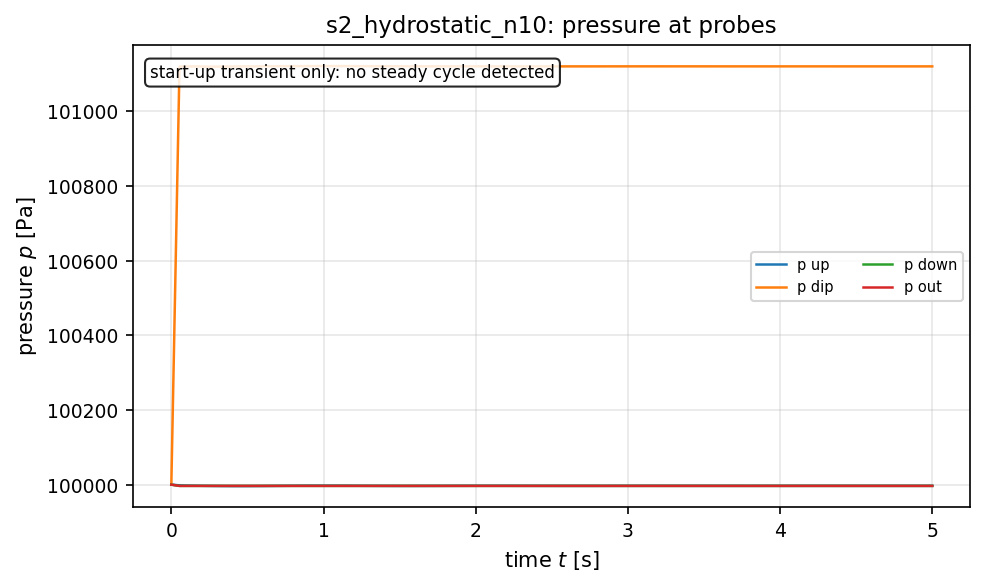
\includegraphics{figures/s2_hydrostatic_n10_pressure.png}
% \caption{Pressure time series at the upstream, dip and downstream
% probes. (s2\_hydrostatic\_n10)}
% \end{figure}

% \begin{figure}
% \centering
% 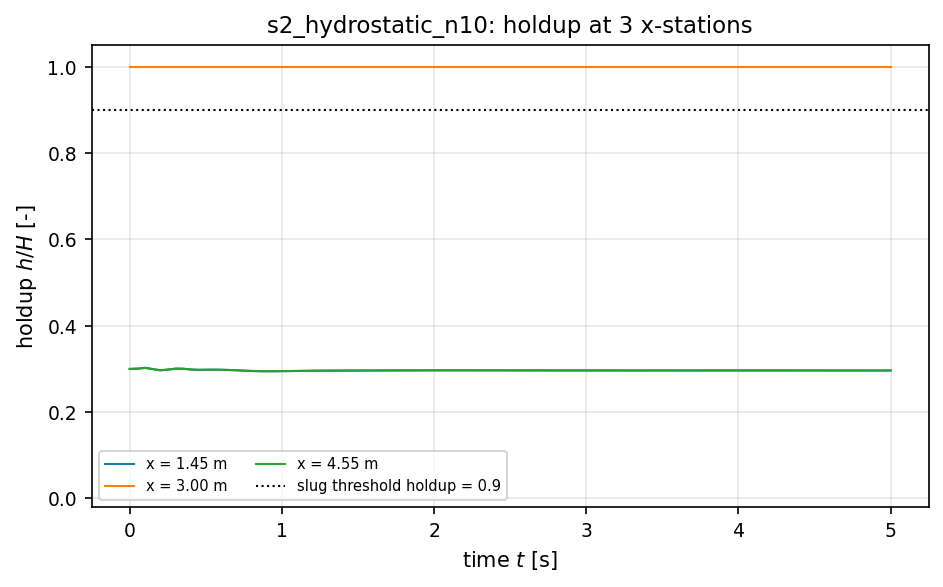
\includegraphics{figures/s2_hydrostatic_n10_holdup_stations.png}
% \caption{Holdup (alpha\_l) at the measurement stations.
% (s2\_hydrostatic\_n10)}
% \end{figure}

% \begin{figure}
% \centering
% 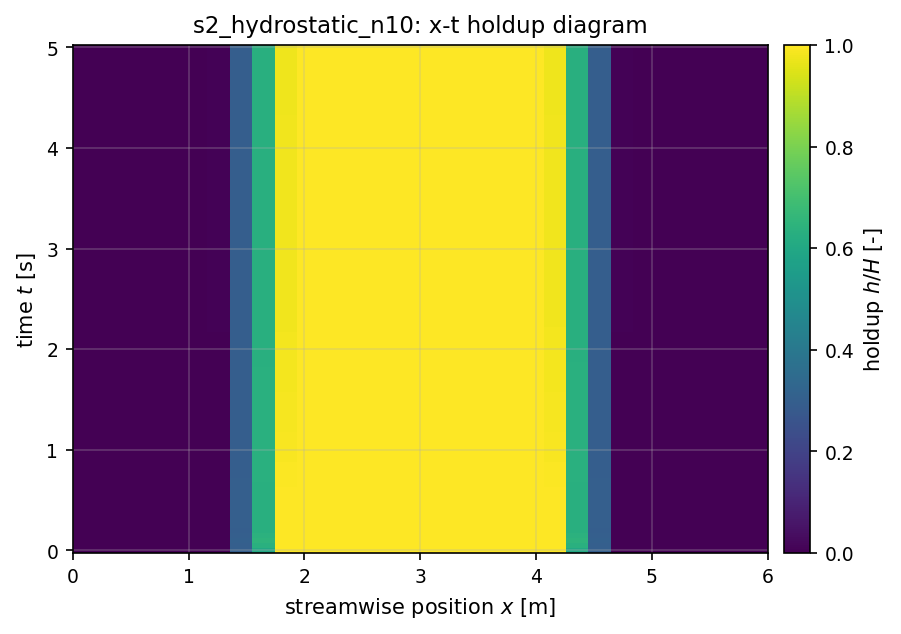
\includegraphics{figures/s2_hydrostatic_n10_xt.png}
% \caption{Space-time diagram of holdup. (s2\_hydrostatic\_n10)}
% \end{figure}

\begin{figure}
\centering
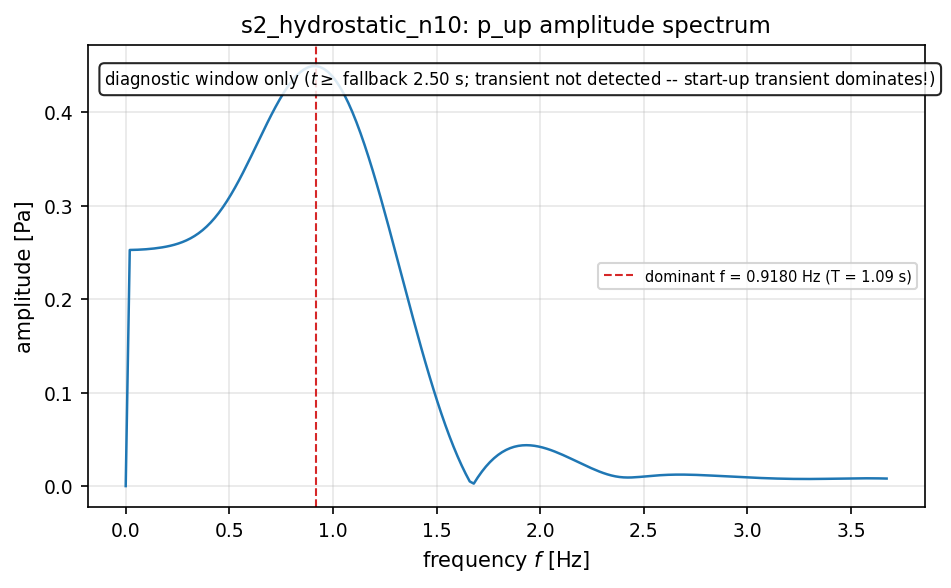
\includegraphics{figures/s2_hydrostatic_n10_fft.png}
\caption{FFT of the upstream pressure.}
\label{fig:fft_pressue}
\end{figure}

% \begin{figure}
% \centering
% 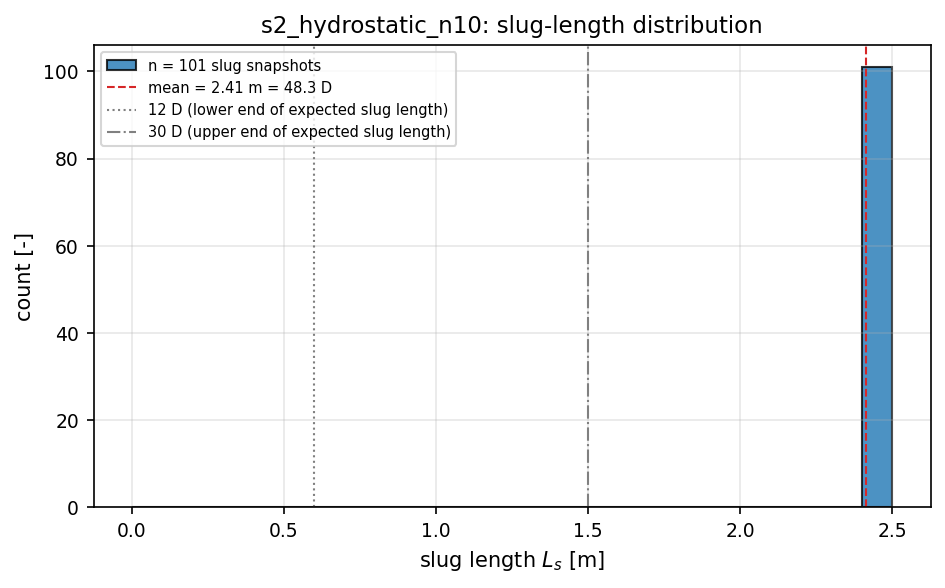
\includegraphics{figures/s2_hydrostatic_n10_slug_hist.png}
% \caption{Histogram of detected slug lengths. (s2\_hydrostatic\_n10)}
% \end{figure}
\begin{figure}[htbp]
\centering
\begin{minipage}{0.48\linewidth}
  \centering
  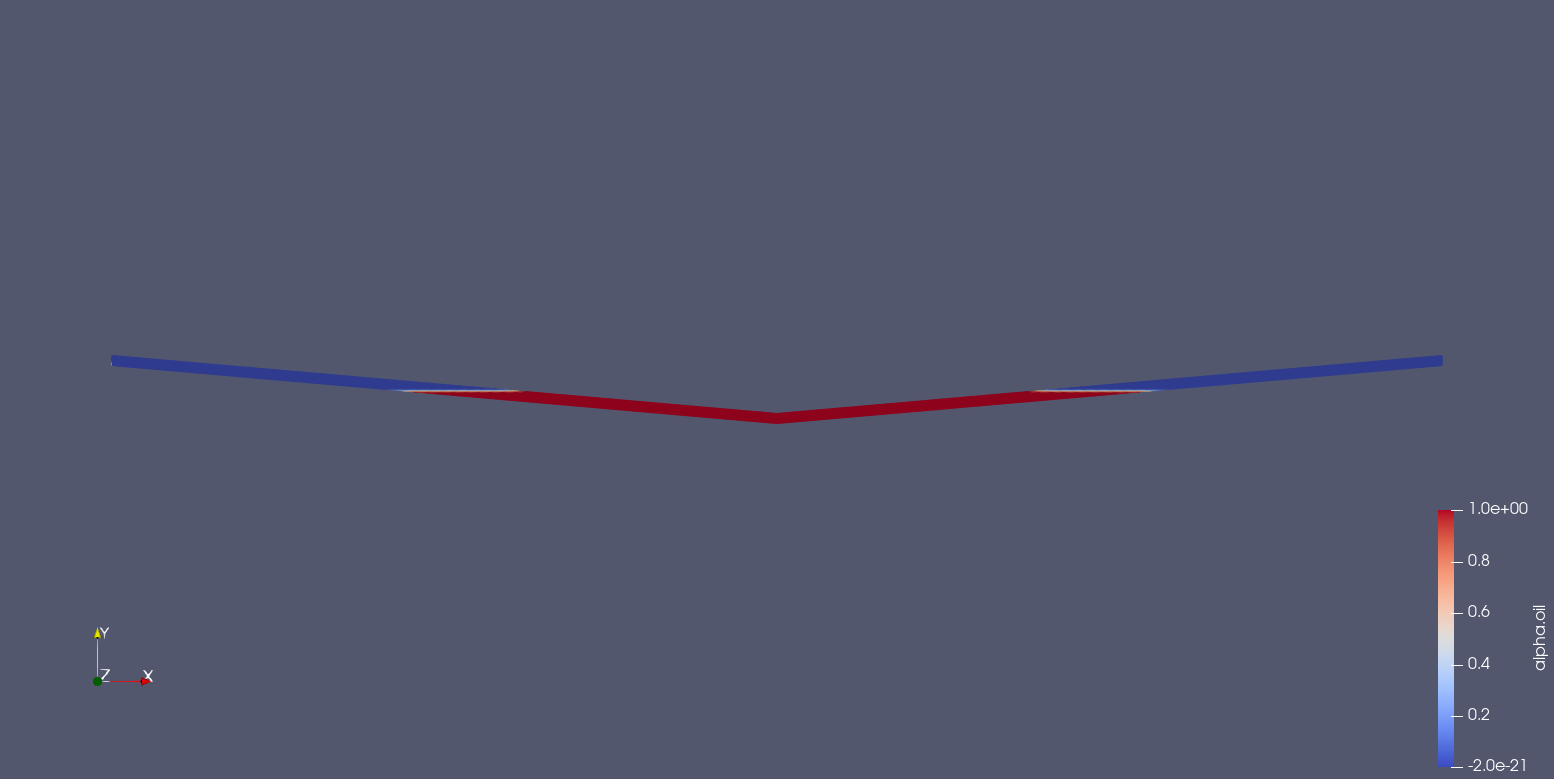
\includegraphics[width=\linewidth]{figures/alpha_oil.png}\\
  \small (a) Liquid fraction $\alpha_l$
\end{minipage}\hfill
\begin{minipage}{0.48\linewidth}
  \centering
  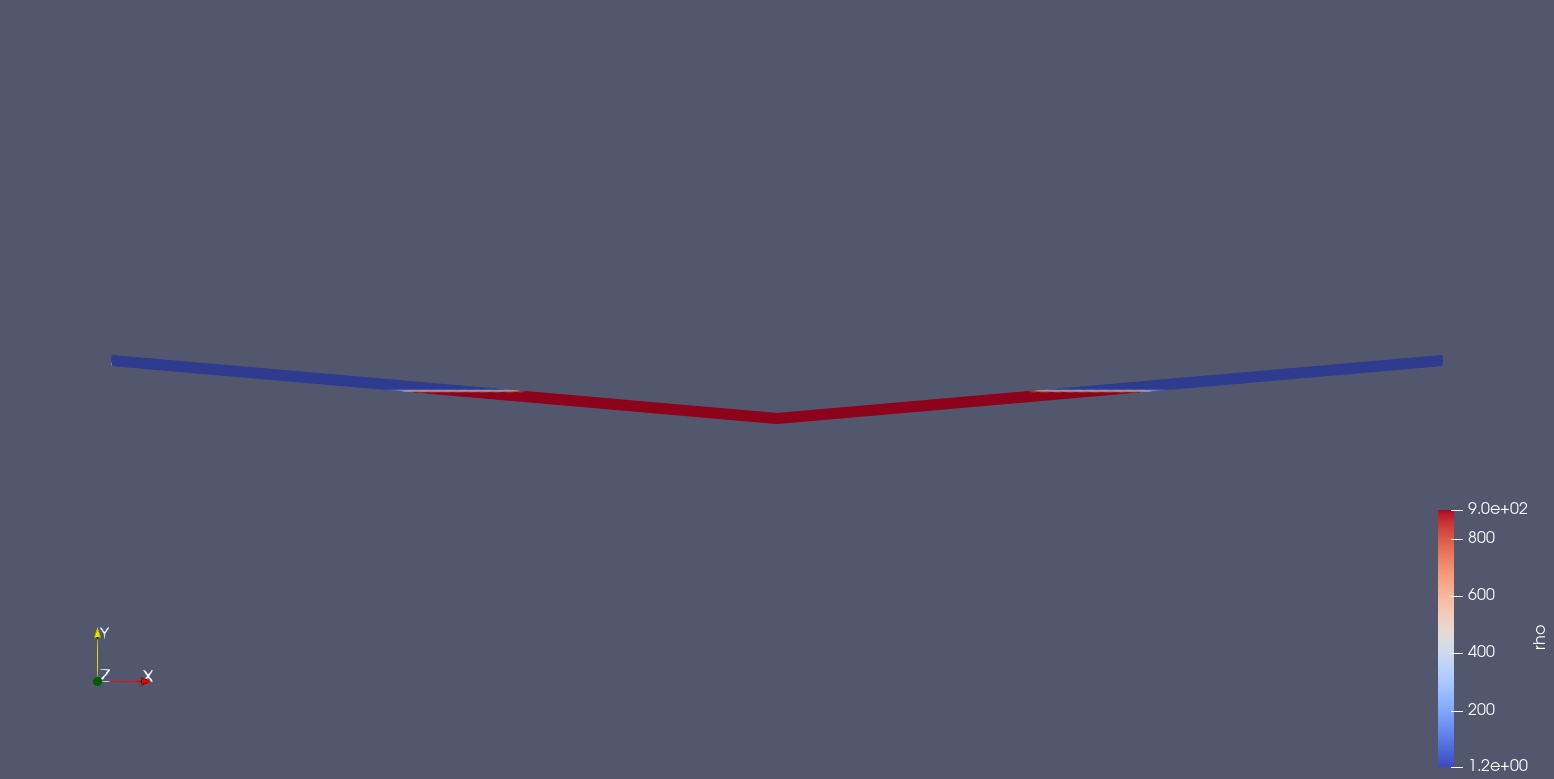
\includegraphics[width=\linewidth]{figures/rho.png}\\
  \small (b) Mixture density $\rho$ [kg/m$^3$]
\end{minipage}

\vspace{4mm}

\begin{minipage}{0.48\linewidth}
  \centering
  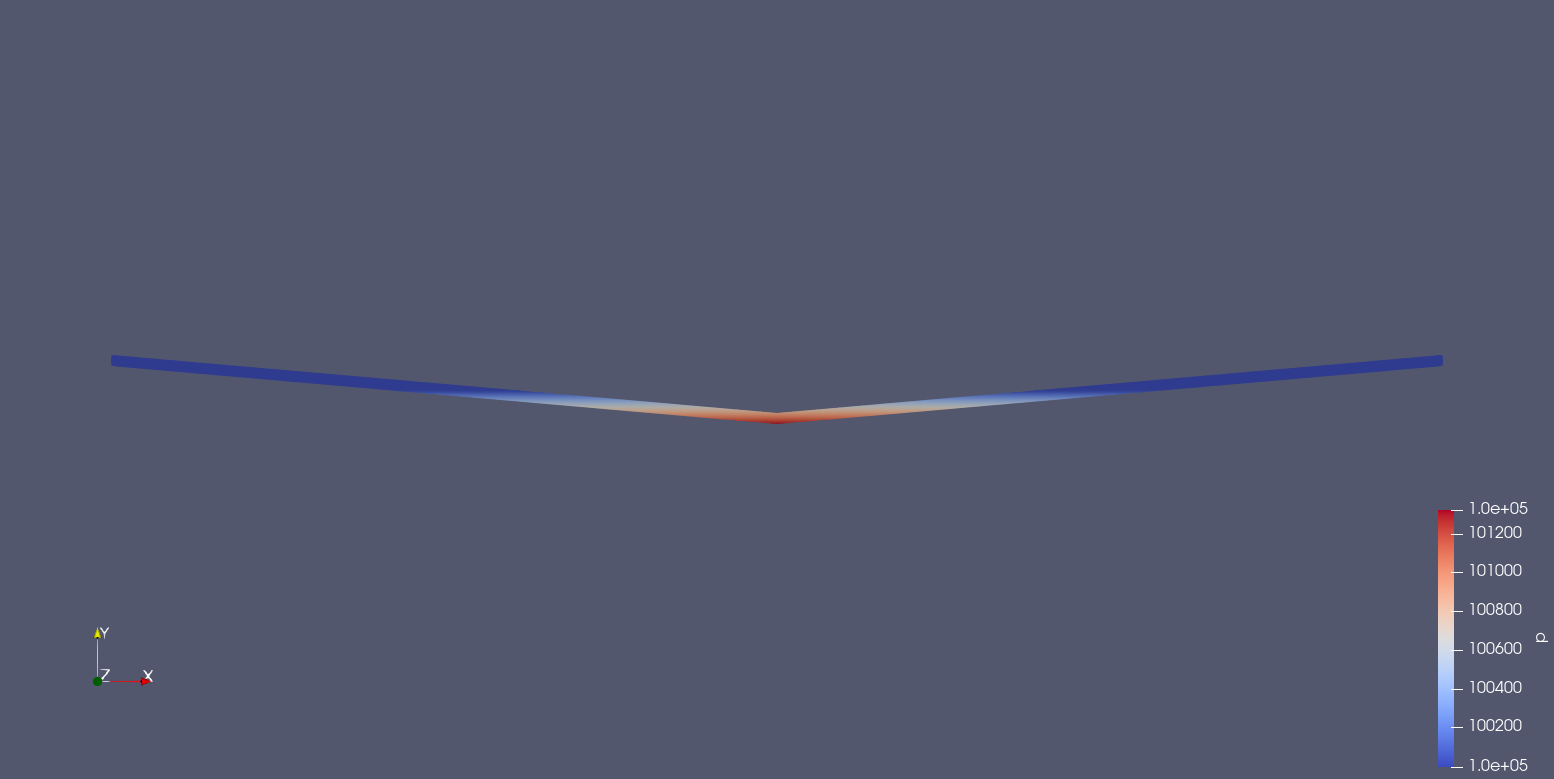
\includegraphics[width=\linewidth]{figures/pressure.png}\\
  \small (c) Pressure $p$ [Pa]
\end{minipage}\hfill
\begin{minipage}{0.48\linewidth}
  \centering
  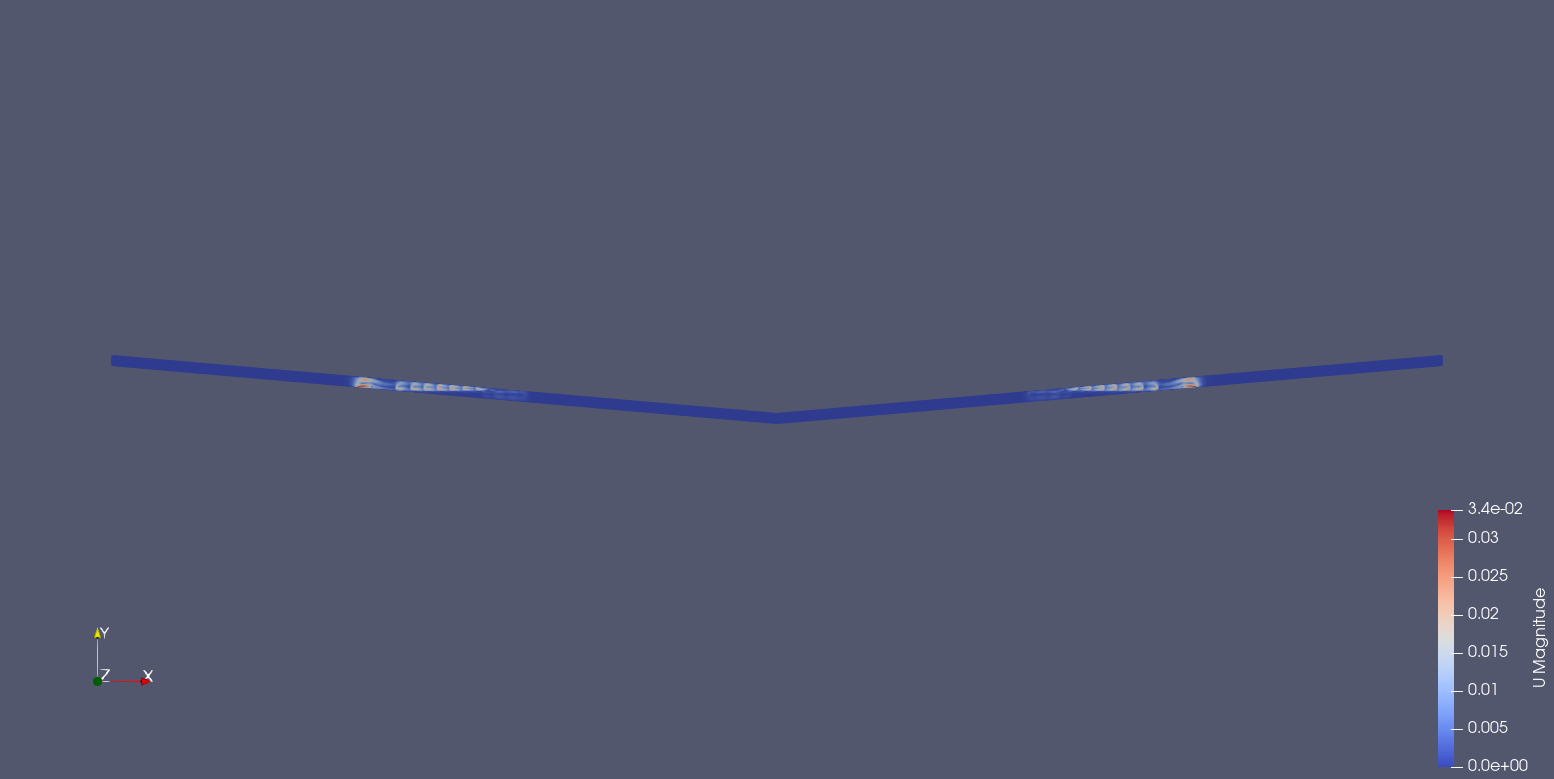
\includegraphics[width=\linewidth]{figures/V.png}\\
  \small (d) Velocity magnitude $|\mathbf{U}|$ [m/s]
\end{minipage}
\caption{Fields at $t = 5$\,s for case \texttt{dip2D\_hydrostatic\_n10}:
flat interface (a), sharp density jump (b), hydrostatic pressure (c) and
residual spurious currents (d).}
\label{fig:fields}
\end{figure}

The interface stays flat and sharp (Fig.~\ref{fig:fields}a,b), the pressure
is hydrostatic (Fig.~\ref{fig:fields}c), and the residual velocity
(Fig.~\ref{fig:fields}d) peaks at $\approx 0.04$\,m/s near the interface. Fig.~\ref{fig:fft_pressue} gives the fourier transforms of the pressure.

\subsection{6.3 Convergence studies}\label{convergence-studies}

The pressure is mesh insensitive with up to 0.01 \% . The spurious current $n=10$ (Spatial mesh division: $D/dx=10$) gives about $0.04 m/s$ while those of $n=20$ gives about 0.038 m/s. 
% No mesh study is complete for the spurious current: n = 10 gives about
% 0.040 m/s and n = 20 about 0.038 m/s (case
% \texttt{dip2D\_hydrostatic\_n20}), i.e.~the parasitic current does
% not decrease with refinement. The sigma = 0 control
% (\texttt{dip2D\_hydrostatic\_nosigma\_n10}) gives the same order, which
% proves the current is not capillary. The pressure itself is
% mesh-insensitive to 0.01 \%.

\subsection{6.4 Critical analysis and limitations}\label{critical-analysis-and-limitations}

\begin{itemize}
\tightlist
\item
  The model is \textbf{2D planar}, not axisymmetric or a circular pipe:
  holdup and slug length are comparable to a pipe.
\item
  The spurious-current criterion
  \(\max|\mathbf U| < 1\,\%\,J_G\) is \textbf{not met}
  (\(\max|\mathbf U| \sim 8\,\%\,J_G\)), and the current persists at all
  tested resolutions. It is not capillary and does not decay, but it is
  only 0.6 \% of the dynamic gas velocities during the release, so it
  does not affect the cycle metrics.
\item
  The gas is close to adiabatic in the baseline; the isothermal twin
  bounds the thermodynamic model-form uncertainty to about 1 \% on the
  start-up peak.
\item
  The gas in-situ Reynolds number is \textasciitilde2.4e3 (transitional
  edge) and the model is laminar: this is an assumption, not a resolved
  turbulence effect.
\end{itemize}

\subsection{6.5 What can be concluded}\label{what-can-be-concluded}

The solver reproduces the hydrostatic state and the
start-up pressure release to within the GCI; compressibility changes the
start-up peak by \textasciitilde1.2 \%; the dip at this operating point
shows weak aperiodic pressure oscillations rather than a converged
slugging cycle (see the main report).

\section{7. Reproduction instructions}\label{reproduction-instructions}

\subsection{7.1 Software environment and dependencies}\label{software-environment-and-dependencies}

\begin{itemize}
\tightlist
\item
  \textbf{OpenFOAM-14} (Foundation build, openfoam.org), solver
  \texttt{foamRun\ -solver\ compressibleVoF}.
\item
  Linux, bash; OpenMPI only for \texttt{NPROC\ \textgreater{}\ 1}.
\item
  Python 3.10+ with \texttt{numpy}, \texttt{pandas},
  \texttt{matplotlib}, \texttt{pyyaml} (project pipeline for visualization).
\item
  \texttt{pandoc} + \texttt{latexmk}/\texttt{pdflatex} only to rebuild
  this report.
\item
  Environment: \texttt{source\ /opt/openfoam14/etc/bashrc}.
\end{itemize}

\subsection{7.2 Step-by-step}\label{step-by-step}

\begin{enumerate}
\def\labelenumi{\arabic{enumi}.}
\tightlist
\item
  Run it in place:
  \texttt{cd\ ./dip2D\_hydrostatic\_n10\ \&\&\ ./Allclean\ \&\&\ ./Allrun}
  (or \texttt{NPROC=12\ ./Allrun}).
\item
  Post-process to VTK:
  \texttt{source\ /opt/openfoam14/etc/bashrc\ \&\&\ foamToVTK\ -latestTime},
  then open \texttt{VTK/*.vtk} in ParaView (colour by \texttt{alpha.oil}
  for the interface).
\end{enumerate}

\section{8. Automation}\label{automation}

\begin{longtable}[]{@{}
  >{\raggedright\arraybackslash}p{(\columnwidth - 4\tabcolsep) * \real{0.3333}}
  >{\raggedright\arraybackslash}p{(\columnwidth - 4\tabcolsep) * \real{0.3333}}
  >{\raggedright\arraybackslash}p{(\columnwidth - 4\tabcolsep) * \real{0.3333}}@{}}
\toprule\noalign{}
\begin{minipage}[b]{\linewidth}\raggedright
script
\end{minipage} & \begin{minipage}[b]{\linewidth}\raggedright
what it does
\end{minipage} & \begin{minipage}[b]{\linewidth}\raggedright
notes
\end{minipage} \\
\midrule\noalign{}
\endhead
\bottomrule\noalign{}
\endlastfoot
\texttt{Allrun} & blockMesh (if needed) + setFields (if present) +
checkMesh + foamRun & serial by default; \texttt{NPROC=12\ ./Allrun} for
MPI; \texttt{-\/-continue} restarts \\
\texttt{Allclean} & removes written times except \texttt{0/},
\texttt{postProcessing/}, \texttt{VTK/}, logs, \texttt{polyMesh} &
idempotent; keeps the setup \\
\texttt{run.sh} & in-place run with metadata recording (case key,
OpenFOAM version, git hash) & used when you want a self-contained case
run \\
\end{longtable}

\section{9. Repository hygiene and organization}\label{repository-hygiene-and-organization}

\begin{itemize}
\tightlist
\item
  Simulation results are precised inside \texttt{.gitignore}
  excludes \texttt{runs/}, \texttt{./*/[0-9]*/},
  \texttt{./*/postProcessing/}, \texttt{./*/VTK/},
  \texttt{./*/log.*}, \texttt{constant/polyMesh}, and LaTeX build
  artefacts.
\item
  This case directory contains only inputs: \texttt{0/},
  \texttt{constant/}, \texttt{system/}, \texttt{Allrun},
  \texttt{Allclean}, \texttt{run.sh}, \texttt{meta.json}, this README.
\item
  All inputs are reproducible from \texttt{../all\_params.yaml}.
\end{itemize}

\section*{References}\label{references}

\noindent [1]--[13]: terrain-slugging literature, VOF/CSF methods, error
estimation and the OpenFOAM-14 documentation.

\medskip

\begin{description}\setlength{\itemsep}{2pt}
\item[{[1]}] Schmidt, Z., Brill, J.P., Beggs, H.D. (1980). Experimental study
of severe slugging in a two-phase-flow pipeline-riser pipe system.
\emph{SPE J.} 20(5), 407-414.
\item[{[2]}] Taitel, Y. (1986). Stability of
severe slugging. \emph{Int. J. Multiphase Flow} 12(2), 203-217.
\item[{[3]}] de Henau, V., Raithby, G.D. (1995a). A transient two-fluid model for the
simulation of slug flow in pipelines - I. Theory. \emph{Int. J.
Multiphase Flow} 21(3), 335-349.
\item[{[4]}] de Henau, V., Raithby, G.D.
(1995b). A transient two-fluid model for the simulation of slug flow in
pipelines - II. Validation. \emph{Int. J. Multiphase Flow} 21(3),
351-363.
\item[{[5]}] de Henau, V., Raithby, G.D. (1995c). A study of
terrain-induced slugging in two-phase flow pipelines. \emph{Int. J.
Multiphase Flow} 21(3), 365-379.
\item[{[6]}] Zuber, N., Findlay, J.A.
(1965). Average volumetric concentration in two-phase flow systems.
\emph{J. Heat Transfer} 87(4), 453-468.
\item[{[7]}] Bendiksen, K.H. (1984). An experimental investigation of the
motion of long bubbles in inclined tubes. \emph{Int. J. Multiphase Flow}
10(4), 467-483.
\item[{[8]}] Hirt, C.W., Nichols, B.D.
(1981). Volume of fluid (VOF) method for the dynamics of free
boundaries. \emph{J. Comput. Phys.} 39, 201-225.
\item[{[9]}] Brackbill,
J.U., Kothe, D.B., Zemach, C. (1992). A continuum method for modeling
surface tension. \emph{J. Comput. Phys.} 100, 335-354.
\item[{[10]}] Rusche,
H. (2002). \emph{Computational fluid dynamics of dispersed two-phase
flows at high phase fractions}. PhD thesis, Imperial College London.
\item[{[11]}] Issa, R.I. (1986). Solution of the implicitly discretised fluid
flow equations by operator-splitting. \emph{J. Comput. Phys.} 62, 40-65.
\item[{[12]}] Celik, I.B., Ghia, U., Roache, P.J., Freitas, C.J., Coleman,
H., Raad, P.E. (2008). Procedure for estimation and reporting of
uncertainty due to discretization in CFD applications. \emph{J. Fluids
Eng.} 130(7), 078001.
\item[{[13]}] OpenFOAM Foundation (2026). OpenFOAM-14,
\url{https://openfoam.org/14}, \url{https://openfoam.org/release/14/} (solver module \texttt{compressibleVoF}).
\end{description}

\end{document}